% !TEX root = ./main.tex
% ^ Tells LaTeX Workshop (Cursor/VSCode) to treat this file as the build root.
% Local-dev build-mode toggle. 1 = handout (all \pause overlays collapsed,
% small PDF), 0 = presentation (each \pause becomes an extra page, for
% live talks). CI overrides this via latexmk -usepretex regardless of what
% it's set to here, so this line only affects local pdflatex/latexmk runs.
\providecommand{\HANDOUT}{1}
% arena_beamer.sty - shared preamble for all ARENA talk decks.
%
% Loaded BEFORE \documentclass (via plain \input, not \usepackage) so that
% it can decide whether to pass `handout` to beamer based on the \HANDOUT
% toggle. The deck pattern is:
%
%   \providecommand{\HANDOUT}{1}              % 1 = handout, 0 = presentation
%   % arena_beamer.sty - shared preamble for all ARENA talk decks.
%
% Loaded BEFORE \documentclass (via plain \input, not \usepackage) so that
% it can decide whether to pass `handout` to beamer based on the \HANDOUT
% toggle. The deck pattern is:
%
%   \providecommand{\HANDOUT}{1}              % 1 = handout, 0 = presentation
%   % arena_beamer.sty - shared preamble for all ARENA talk decks.
%
% Loaded BEFORE \documentclass (via plain \input, not \usepackage) so that
% it can decide whether to pass `handout` to beamer based on the \HANDOUT
% toggle. The deck pattern is:
%
%   \providecommand{\HANDOUT}{1}              % 1 = handout, 0 = presentation
%   \input{../../arena_beamer.sty}
%   ... deck-local macros ...
%   \begin{document} ... \end{document}
%
% CI overrides the deck's local toggle via latexmk's -usepretex flag, which
% \def's \HANDOUT before main.tex starts. The \providecommand below is a
% safety default if neither the deck nor CI set anything.

\providecommand{\HANDOUT}{1}
\ifnum\HANDOUT=1
  \PassOptionsToClass{handout}{beamer}
\fi
\documentclass[10pt,a4paper]{beamer}

\RequirePackage[latin1]{inputenc}
\RequirePackage{amsmath}
\RequirePackage{amsfonts}
\RequirePackage{amssymb}
\RequirePackage{graphicx}
\RequirePackage{ulem}
\RequirePackage{algorithm2e}
\RequirePackage{algpseudocode}
\RequirePackage{diffcoeff}
\RequirePackage{xcolor}
\RequirePackage{tikz}
\RequirePackage{cancel}
\RequirePackage{pgfplots}
\RequirePackage{background}
\RequirePackage{stmaryrd}
\RequirePackage{subcaption}
\RequirePackage{ifthen}
\RequirePackage{listings}
\RequirePackage{hyperref}

\usetheme{Madrid}

\hypersetup{
    colorlinks=true,
    linkcolor=white,
    filecolor=magenta,
    urlcolor=cyan,
}
\urlstyle{same}

\DeclareMathOperator*{\argmin}{\arg\!\min}
\DeclareMathOperator*{\argmax}{arg\,max}

\usetikzlibrary{calc, fadings, decorations.pathreplacing, automata, positioning, arrows, shapes.geometric, arrows.meta, positioning, fit, backgrounds}

% Generic math/style macros used across decks.
% Anything chapter-specific (state space, reward set, etc.) lives in the
% deck's own main.tex, not here.
\newcommand{\Ex}{\mathbb{E}}
\newcommand{\red}[1]{\textcolor{red}{#1}}
\newcommand{\bth}{{\boldsymbol{\theta}}}

% PyTorch code listing style.
\definecolor{codegreen}{rgb}{0,0.5,0}
\definecolor{codegray}{rgb}{0.4,0.4,0.4}
\definecolor{codepurple}{rgb}{0.55,0.0,0.55}
\definecolor{codeblue}{rgb}{0.0,0.0,0.6}

\lstdefinestyle{pystyle}{
    basicstyle=\ttfamily\scriptsize,
    keywordstyle=\color{codeblue}\bfseries,
    commentstyle=\color{codegreen}\itshape,
    stringstyle=\color{codepurple},
    numberstyle=\tiny\color{codegray},
    breaklines=true,
    showstringspaces=false,
    language=Python,
    morekeywords={self, nn, torch, Tensor},
    columns=fullflexible,
    keepspaces=true,
}
\lstset{style=pystyle}

% Decks set their own \graphicspath after \usepackage{arena_beamer}, but
% default to img/ so plain \includegraphics works without ceremony.
\graphicspath{{img/}}

% Falls back to a labeled placeholder box if the image file isn't present.
% Usage: \imgorplaceholder{0.6\linewidth}{filename-no-ext}{Caption shown if missing}
\newcommand{\imgorplaceholder}[3]{%
    \IfFileExists{img/#2.png}{\includegraphics[width=#1]{#2}}{%
    \IfFileExists{img/#2.jpg}{\includegraphics[width=#1]{#2}}{%
    \IfFileExists{img/#2.pdf}{\includegraphics[width=#1]{#2}}{%
    \IfFileExists{img/#2.svg}{\includegraphics[width=#1]{#2}}{%
        \fbox{\parbox[c][0.45\textheight][c]{#1}{\centering \textit{[image: #3]}\\\scriptsize drop \texttt{img/#2.(png|jpg|pdf)}}}%
    }}}}%
}

\endinput

%   ... deck-local macros ...
%   \begin{document} ... \end{document}
%
% CI overrides the deck's local toggle via latexmk's -usepretex flag, which
% \def's \HANDOUT before main.tex starts. The \providecommand below is a
% safety default if neither the deck nor CI set anything.

\providecommand{\HANDOUT}{1}
\ifnum\HANDOUT=1
  \PassOptionsToClass{handout}{beamer}
\fi
\documentclass[10pt,a4paper]{beamer}

\RequirePackage[latin1]{inputenc}
\RequirePackage{amsmath}
\RequirePackage{amsfonts}
\RequirePackage{amssymb}
\RequirePackage{graphicx}
\RequirePackage{ulem}
\RequirePackage{algorithm2e}
\RequirePackage{algpseudocode}
\RequirePackage{diffcoeff}
\RequirePackage{xcolor}
\RequirePackage{tikz}
\RequirePackage{cancel}
\RequirePackage{pgfplots}
\RequirePackage{background}
\RequirePackage{stmaryrd}
\RequirePackage{subcaption}
\RequirePackage{ifthen}
\RequirePackage{listings}
\RequirePackage{hyperref}

\usetheme{Madrid}

\hypersetup{
    colorlinks=true,
    linkcolor=white,
    filecolor=magenta,
    urlcolor=cyan,
}
\urlstyle{same}

\DeclareMathOperator*{\argmin}{\arg\!\min}
\DeclareMathOperator*{\argmax}{arg\,max}

\usetikzlibrary{calc, fadings, decorations.pathreplacing, automata, positioning, arrows, shapes.geometric, arrows.meta, positioning, fit, backgrounds}

% Generic math/style macros used across decks.
% Anything chapter-specific (state space, reward set, etc.) lives in the
% deck's own main.tex, not here.
\newcommand{\Ex}{\mathbb{E}}
\newcommand{\red}[1]{\textcolor{red}{#1}}
\newcommand{\bth}{{\boldsymbol{\theta}}}

% PyTorch code listing style.
\definecolor{codegreen}{rgb}{0,0.5,0}
\definecolor{codegray}{rgb}{0.4,0.4,0.4}
\definecolor{codepurple}{rgb}{0.55,0.0,0.55}
\definecolor{codeblue}{rgb}{0.0,0.0,0.6}

\lstdefinestyle{pystyle}{
    basicstyle=\ttfamily\scriptsize,
    keywordstyle=\color{codeblue}\bfseries,
    commentstyle=\color{codegreen}\itshape,
    stringstyle=\color{codepurple},
    numberstyle=\tiny\color{codegray},
    breaklines=true,
    showstringspaces=false,
    language=Python,
    morekeywords={self, nn, torch, Tensor},
    columns=fullflexible,
    keepspaces=true,
}
\lstset{style=pystyle}

% Decks set their own \graphicspath after \usepackage{arena_beamer}, but
% default to img/ so plain \includegraphics works without ceremony.
\graphicspath{{img/}}

% Falls back to a labeled placeholder box if the image file isn't present.
% Usage: \imgorplaceholder{0.6\linewidth}{filename-no-ext}{Caption shown if missing}
\newcommand{\imgorplaceholder}[3]{%
    \IfFileExists{img/#2.png}{\includegraphics[width=#1]{#2}}{%
    \IfFileExists{img/#2.jpg}{\includegraphics[width=#1]{#2}}{%
    \IfFileExists{img/#2.pdf}{\includegraphics[width=#1]{#2}}{%
    \IfFileExists{img/#2.svg}{\includegraphics[width=#1]{#2}}{%
        \fbox{\parbox[c][0.45\textheight][c]{#1}{\centering \textit{[image: #3]}\\\scriptsize drop \texttt{img/#2.(png|jpg|pdf)}}}%
    }}}}%
}

\endinput

%   ... deck-local macros ...
%   \begin{document} ... \end{document}
%
% CI overrides the deck's local toggle via latexmk's -usepretex flag, which
% \def's \HANDOUT before main.tex starts. The \providecommand below is a
% safety default if neither the deck nor CI set anything.

\providecommand{\HANDOUT}{1}
\ifnum\HANDOUT=1
  \PassOptionsToClass{handout}{beamer}
\fi
\documentclass[10pt,a4paper]{beamer}

\RequirePackage[latin1]{inputenc}
\RequirePackage{amsmath}
\RequirePackage{amsfonts}
\RequirePackage{amssymb}
\RequirePackage{graphicx}
\RequirePackage{ulem}
\RequirePackage{algorithm2e}
\RequirePackage{algpseudocode}
\RequirePackage{diffcoeff}
\RequirePackage{xcolor}
\RequirePackage{tikz}
\RequirePackage{cancel}
\RequirePackage{pgfplots}
\RequirePackage{background}
\RequirePackage{stmaryrd}
\RequirePackage{subcaption}
\RequirePackage{ifthen}
\RequirePackage{listings}
\RequirePackage{hyperref}

\usetheme{Madrid}

\hypersetup{
    colorlinks=true,
    linkcolor=white,
    filecolor=magenta,
    urlcolor=cyan,
}
\urlstyle{same}

\DeclareMathOperator*{\argmin}{\arg\!\min}
\DeclareMathOperator*{\argmax}{arg\,max}

\usetikzlibrary{calc, fadings, decorations.pathreplacing, automata, positioning, arrows, shapes.geometric, arrows.meta, positioning, fit, backgrounds}

% Generic math/style macros used across decks.
% Anything chapter-specific (state space, reward set, etc.) lives in the
% deck's own main.tex, not here.
\newcommand{\Ex}{\mathbb{E}}
\newcommand{\red}[1]{\textcolor{red}{#1}}
\newcommand{\bth}{{\boldsymbol{\theta}}}

% PyTorch code listing style.
\definecolor{codegreen}{rgb}{0,0.5,0}
\definecolor{codegray}{rgb}{0.4,0.4,0.4}
\definecolor{codepurple}{rgb}{0.55,0.0,0.55}
\definecolor{codeblue}{rgb}{0.0,0.0,0.6}

\lstdefinestyle{pystyle}{
    basicstyle=\ttfamily\scriptsize,
    keywordstyle=\color{codeblue}\bfseries,
    commentstyle=\color{codegreen}\itshape,
    stringstyle=\color{codepurple},
    numberstyle=\tiny\color{codegray},
    breaklines=true,
    showstringspaces=false,
    language=Python,
    morekeywords={self, nn, torch, Tensor},
    columns=fullflexible,
    keepspaces=true,
}
\lstset{style=pystyle}

% Decks set their own \graphicspath after \usepackage{arena_beamer}, but
% default to img/ so plain \includegraphics works without ceremony.
\graphicspath{{img/}}

% Falls back to a labeled placeholder box if the image file isn't present.
% Usage: \imgorplaceholder{0.6\linewidth}{filename-no-ext}{Caption shown if missing}
\newcommand{\imgorplaceholder}[3]{%
    \IfFileExists{img/#2.png}{\includegraphics[width=#1]{#2}}{%
    \IfFileExists{img/#2.jpg}{\includegraphics[width=#1]{#2}}{%
    \IfFileExists{img/#2.pdf}{\includegraphics[width=#1]{#2}}{%
    \IfFileExists{img/#2.svg}{\includegraphics[width=#1]{#2}}{%
        \fbox{\parbox[c][0.45\textheight][c]{#1}{\centering \textit{[image: #3]}\\\scriptsize drop \texttt{img/#2.(png|jpg|pdf)}}}%
    }}}}%
}

\endinput


% Deck-local macros.
\newcommand{\R}{\mathbb{R}}

\begin{document}

\title[{[0.3] Optimization, Hyperparameters, and Scale}]
{{[0.3] Optimization, Hyperparameters, and Scale}}

\author[David Quarel]
{David Quarel}

\institute[ARENA]
{
  ARENA
}

\date[\today]
{\today}

\frame{\titlepage}

% ------------------------------------------------------------
\begin{frame}
\frametitle{What's today about?}
\begin{itemize}
    \item Yesterday: you built ResNet34. Today: we explore what the optimizer does,
    build some from scratch, and train with them.
    \pause
    \item The road there:
    \begin{enumerate}
        \item Optimizers --- SGD, momentum, Adam, AdamW, and \emph{why}
        they exist.
        \pause
        \item Experiment tracking + hyperparameter sweeps with Weights \&
        Biases.
        \pause
        \item Distributed training --- when one GPU isn't enough.
    \end{enumerate}
\end{itemize}
\end{frame}

% ------------------------------------------------------------
\begin{frame}[fragile]
    \frametitle{The training loop}
    \begin{itemize}
        \item Same four steps every iteration: \textit{forward, loss, backward, step}.
    \end{itemize}
    \begin{block}{}
    \begin{lstlisting}[basicstyle=\small\ttfamily]
    for x, y in dataloader:                
        y_hat = model(x)                   
        loss = loss_fn(y,y_hat)
        loss.backward()          
        optimizer.step()         # Build this today
        optimizer.zero_grad()    # Build this today
    \end{lstlisting}
    \end{block}
    \pause
    \begin{itemize}
        \item \texttt{loss.backward()} fills \texttt{.grad} on every parameter via
        autograd.
        \pause
        \item \texttt{optimizer.step()} applies an update rule
        (e.g.\ Adam: momentum + per-parameter adaptive learning rate).
        \pause
        \item \texttt{zero\_grad()} before backward: gradients \textbf{accumulate}
        by default in PyTorch.
    \end{itemize}
    \end{frame}


% ------------------------------------------------------------
\begin{frame}
\frametitle{Loss landscapes \& why this is hard}
\begin{itemize}
    \item Loss is a function $\mathcal{L} : \R^d \to \R$ over millions of
    parameters. We never see the full thing --- only 1D/2D slices through it.
    \pause
    \item Common pathologies:
    \begin{itemize}
        \item \textbf{Ravines:} one direction much steeper than another.
        Naive SGD oscillates across, crawls along.
        \pause
        \item \textbf{Saddle points:} gradient is zero but you're not at a
        minimum.
        \pause
        \item \textbf{Plateaus:} gradient is tiny; nothing moves.
    \end{itemize}
\end{itemize}
\begin{center}
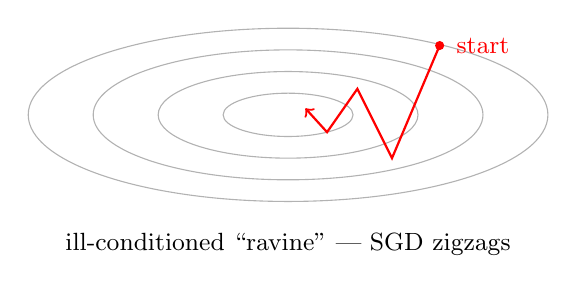
\begin{tikzpicture}[scale=0.55]
    % Ravine: nested ellipses, very elongated
    \foreach \r in {1, 2, 3, 4} {
        \draw[gray!60] (0,0) ellipse ({3*\r/2} and {\r/2});
    }
    \fill[red] (3.5,1.6) circle (3pt);
    % Zigzag SGD path
    \draw[->, red, thick] (3.5,1.6) -- (2.4,-1.0) -- (1.6,0.6) -- (0.9,-0.4) -- (0.4,0.15);
    \node[red, font=\small] at (4.5,1.6) {start};
    \node[font=\small] at (0,-3) {ill-conditioned ``ravine'' --- SGD zigzags};
\end{tikzpicture}
\end{center}
\end{frame}

% ------------------------------------------------------------
\begin{frame}
\frametitle{Gradient descent recap}
\begin{block}{Gradient descent}
    $$ \theta_{t+1} = \theta_t - \alpha\, \nabla_\theta \mathcal{L}(\theta_t) $$
\end{block}
\begin{itemize}
    \pause
    \item Learning rate $\alpha$ is the single most important hyperparameter.
    Too high $\to$ divergence; too low $\to$ glacial progress.
    \pause
    \item In practice we don't compute $\nabla \mathcal{L}$ on the full
    dataset --- we use \textbf{batches}. The gradient becomes a noisy
    estimate, but each step is much cheaper.
    \pause
    \item If the batch size is too large, one can do several forward passes
    over mini-batches and accumulate gradients to emulate a larger batch size.
    \pause
    \item \textbf{Batch size:}
    \begin{itemize}
        \item Larger $\to$ (+) lower-variance gradient, better GPU utilization
        \item Larger $\to$ (-) more memory, fewer optimizer steps per epoch,
        often worse generalization at scale
    \end{itemize}
\end{itemize}
\end{frame}

% ------------------------------------------------------------
\begin{frame}[fragile]
\begin{block}{SGD}
$$ \theta_{t+1} = \theta_t - \alpha\, g_t $$
\end{block}
\begin{block}{}
\begin{lstlisting}[basicstyle=\normalsize\ttfamily]
class SGD(Optimizer):
    def __init__(self, params, lr):
        self.params = list(params)
        self.lr = lr

    @torch.no_grad()
    def step(self):
        for p in self.params:
            p = p - self.lr * p.grad  # SGD update

    def zero_grad(self):
        for p in self.params:
            p.grad.zero_()
\end{lstlisting}
\end{block}
\end{frame}

% ------------------------------------------------------------
\begin{frame}
\frametitle{Momentum}
\begin{block}{SGD with momentum}
\vspace{-0.3cm}
\begin{align*}
    v_{t+1} &= \mu\, v_t + \nabla_\theta \mathcal{L}(\theta_t) \\
    \theta_{t+1} &= \theta_t - \alpha\, v_{t+1}
\end{align*}
\end{block}
\begin{itemize}
    \pause
    \item $v_t$ is an exponentially weighted moving average of past gradients,
    decayed by $\mu \in [0,1)$ (typically $0.9$).
    \pause
    \item In a ravine, gradient directions across the ravine \emph{cancel}
    on average; directions along it \emph{accumulate}. Smooth, fast progress
    toward the minimum.
    \pause
    \item Equivalent picture: a ball with mass rolling down the landscape.
    Reaches a \textit{terminal velocity} along consistent directions.
    \pause
    \item \href{https://distill.pub/2017/momentum/}{distill.pub/2017/momentum}
    has a beautiful interactive on this.
\end{itemize}
\end{frame}

% ------------------------------------------------------------
\begin{frame}
\frametitle{RMSprop}
\begin{block}{RMSprop}
\vspace{-0.3cm}
\begin{align*}
    s_{t+1} &= \beta\, s_t + (1-\beta)\, \big(\nabla_\theta \mathcal{L}\big)^2 \\
    \theta_{t+1} &= \theta_t - \alpha\, \frac{\nabla_\theta \mathcal{L}}{\sqrt{s_{t+1}} + \varepsilon}
\end{align*}
\end{block}
\begin{itemize}
    \pause
    \item $s_t$ is a moving average of squared gradients (per-parameter).
    \pause
    \item Effect: each parameter gets its own \textbf{adaptive learning rate}.
    Parameters with large historical gradients get smaller updates;
    parameters with tiny gradients get amplified.
    \pause
    \item Implicitly handles ill-conditioning --- it's a cheap, online
    approximation of dividing by the diagonal of the Hessian.
    \pause
    \item \textbf{Memory cost:} $s_t$ is parameter-sized $\Rightarrow$ 2$\times$
    memory vs SGD.
\end{itemize}
\end{frame}

% ------------------------------------------------------------
\begin{frame}
\frametitle{Adam}
\begin{block}{Adam}
\vspace{-0.3cm}
\begin{align*}
    m_{t+1} &= \beta_1 m_t + (1-\beta_1)\, \nabla \mathcal{L}      &&\text{(first moment)} \\
    v_{t+1} &= \beta_2 v_t + (1-\beta_2)\, (\nabla \mathcal{L})^2  &&\text{(second moment)} \\
    \hat{m}_{t+1} &= m_{t+1} / (1 - \beta_1^{t+1})                 &&\text{(bias correction)} \\
    \hat{v}_{t+1} &= v_{t+1} / (1 - \beta_2^{t+1})                 \\
    \theta_{t+1} &= \theta_t - \alpha\, \hat{m}_{t+1} / (\sqrt{\hat{v}_{t+1}} + \varepsilon)
\end{align*}
\end{block}
\begin{itemize}
    \pause
    \item \textbf{Momentum + RMSprop + bias correction}, all at once.
    \pause
    \item Defaults: $\beta_1 = 0.9$, $\beta_2 = 0.999$, $\varepsilon = 10^{-8}$.
    These usually just work.
    \pause
    \item Bias correction matters early in training when $m, v$ are still
    near zero --- without it the first few steps are tiny.
    \pause
    \item \textbf{Memory cost:} $m_t$ \emph{and} $v_t$ are both parameter-sized
    $\Rightarrow$ 3$\times$ memory vs SGD.
\end{itemize}
\end{frame}

% ------------------------------------------------------------
\begin{frame}
\frametitle{Adam vs AdamW: the weight-decay subtlety}
\begin{itemize}
    \item \textbf{Naive weight decay:} add $\tfrac{\lambda}{2}\|\theta\|^2$ to
    the loss. Looks innocent, but for adaptive methods, the L2 gradient
    $\lambda \theta$ gets divided by $\sqrt{\hat{v}_t}$ along with everything
    else --- so parameters with large historical gradients are decayed
    \emph{less}. Not what you want.
    \pause
\end{itemize}
\begin{block}{AdamW: decoupled weight decay}
    $$ \theta_{t+1} = \theta_t - \alpha\, \hat{m}_{t+1}/(\sqrt{\hat{v}_{t+1}}+\varepsilon) - \alpha\, \lambda\, \theta_t $$
\end{block}
\begin{itemize}
    \pause
    \item The $\lambda \theta$ term sits \textit{outside} the adaptive scaling
    --- every parameter shrinks toward zero by the same relative amount each
    step.
    \pause
    \item In practice: just use \texttt{AdamW}.
\end{itemize}
\end{frame}

% ------------------------------------------------------------
\begin{frame}[fragile]
\frametitle{Schedules \& parameter groups}
\begin{itemize}
    \item Fixed LR is fine for toy problems. Real training uses a
    \textbf{schedule}: warmup (linear ramp from 0) + decay (cosine or linear).
\end{itemize}
\begin{center}
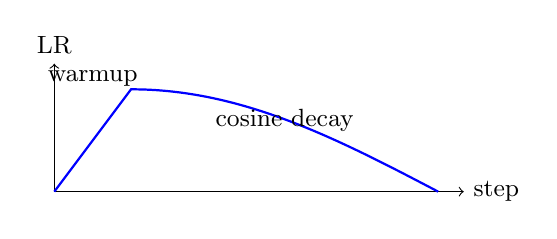
\begin{tikzpicture}[scale=0.65]
    \draw[->] (0,0) -- (8,0) node[right, font=\small] {step};
    \draw[->] (0,0) -- (0,2.5) node[above, font=\small] {LR};
    \draw[thick, blue] (0,0) -- (1.5,2) -- plot[smooth, domain=1.5:7.5] ({\x}, {2*cos((\x-1.5)*15)});
    \node[font=\small] at (0.75, 2.2) {warmup};
    \node[font=\small] at (4.5, 1.4) {cosine decay};
\end{tikzpicture}
\end{center}
\begin{itemize}
    \item \textbf{Parameter groups:} different learning rates for different
    parts of the model. Common in fine-tuning (slow backbone, fast head):
\end{itemize}
\begin{block}{}
\begin{lstlisting}
optimizer = torch.optim.AdamW([
    {"params": backbone.parameters(), "lr": 1e-5, "weight_decay": 0.01},
    {"params": head.parameters(),     "lr": 1e-3, "weight_decay": 0.0},
])
\end{lstlisting}
\end{block}
\end{frame}

% ------------------------------------------------------------
\begin{frame}[fragile]
    \frametitle{Why track experiments? Weights \& Biases}
    \begin{itemize}
        \item WandB is the de-facto tool: can easily track and log loss, accuracy etc. 
        while the model is training
    \end{itemize}
    
    \begin{figure}[h]
        \centering
        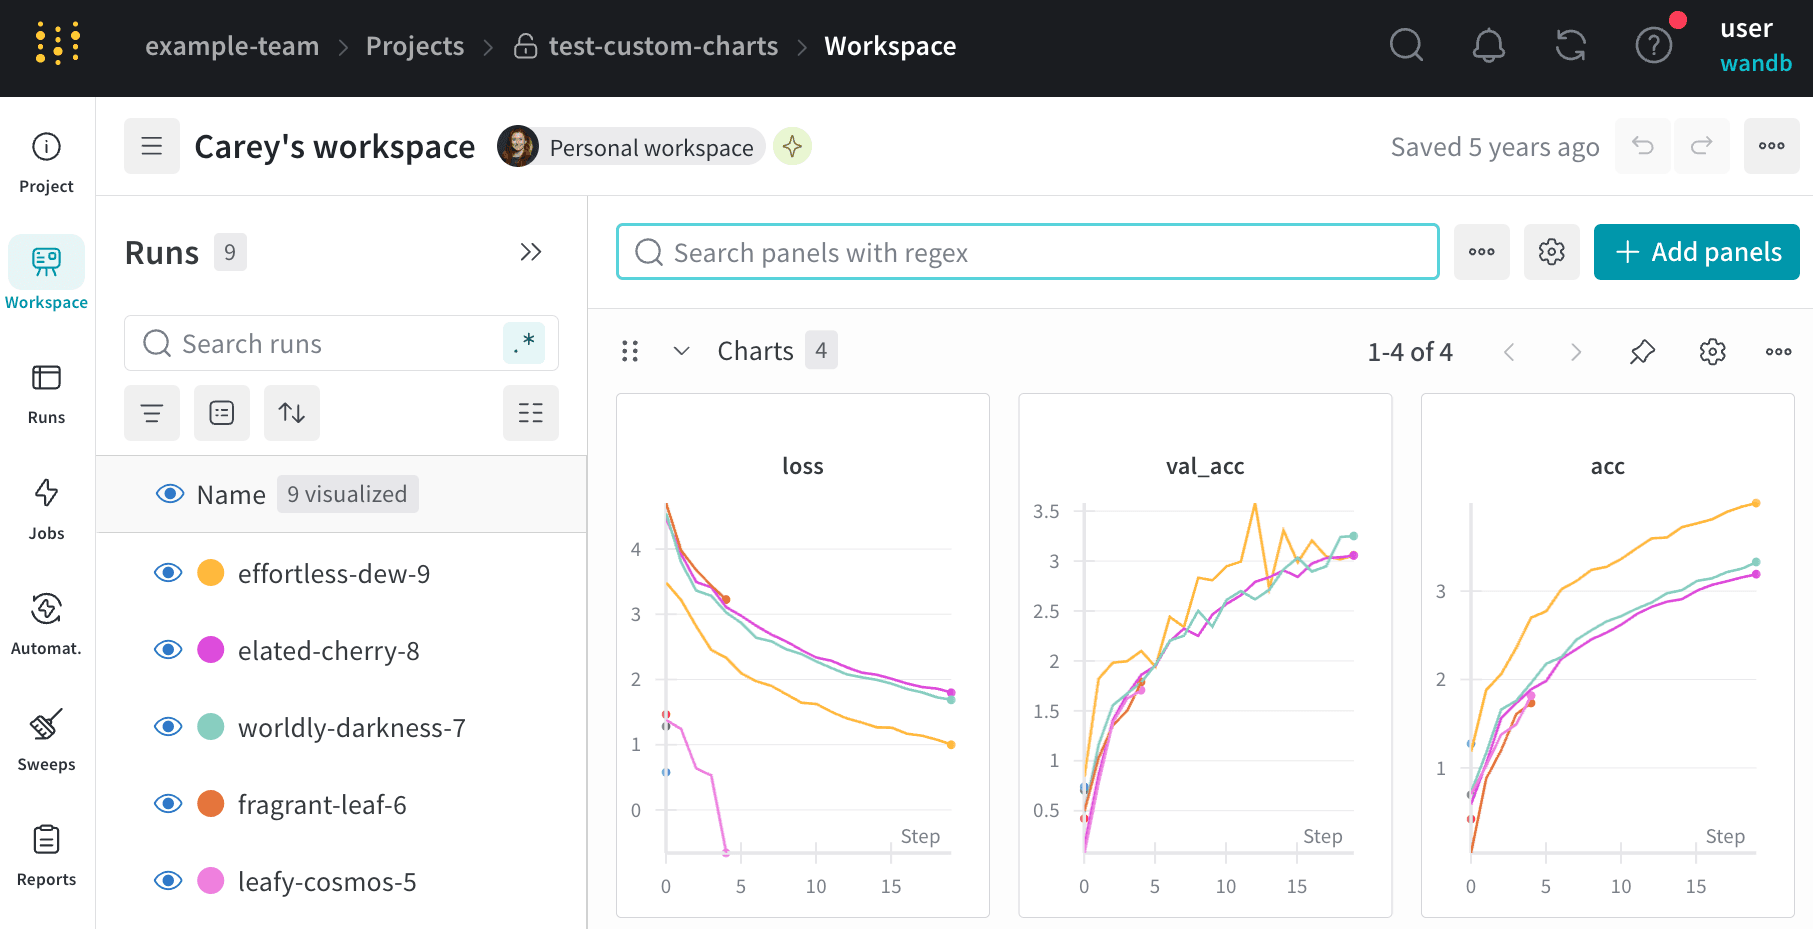
\includegraphics[width=0.8\textwidth]{img/wandb_dashboard.png}
        % image taken from https://docs.wandb.ai/models/track/project-page
        \label{fig:wandb}
    \end{figure}
    
    \end{frame}

% % ------------------------------------------------------------
% \begin{frame}
% \frametitle{Hyperparameter sweeps: grid vs random vs Bayes}
% \begin{center}
%     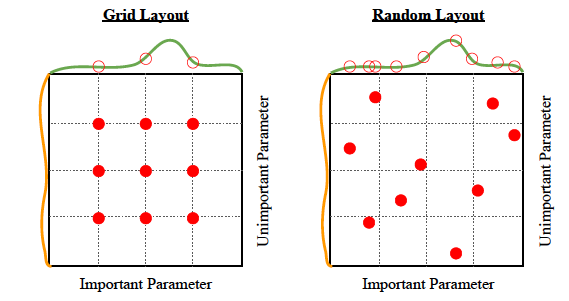
\includegraphics[width=0.6\linewidth]{grid_vs_random}
% \end{center}
% \pause
% \begin{itemize}
%     \item \textbf{Random} is almost always better than grid. In high
%     dimensions, only a few hyperparameters actually matter; grid wastes
%     points on the others. Random gets you more samples along each axis for
%     the same budget.
%     \pause
%     \item \textbf{Bayesian} (Bayes / Hyperband / BOHB): builds a surrogate
%     model of the objective, picks the next config to evaluate. Pays off
%     when one evaluation is expensive (\textit{hours}, not seconds).
%     \pause
%     \item WandB has built-in sweep support: write a 10-line YAML, hit go.
% \end{itemize}
% \end{frame}

\begin{frame}[plain]
    \centering
    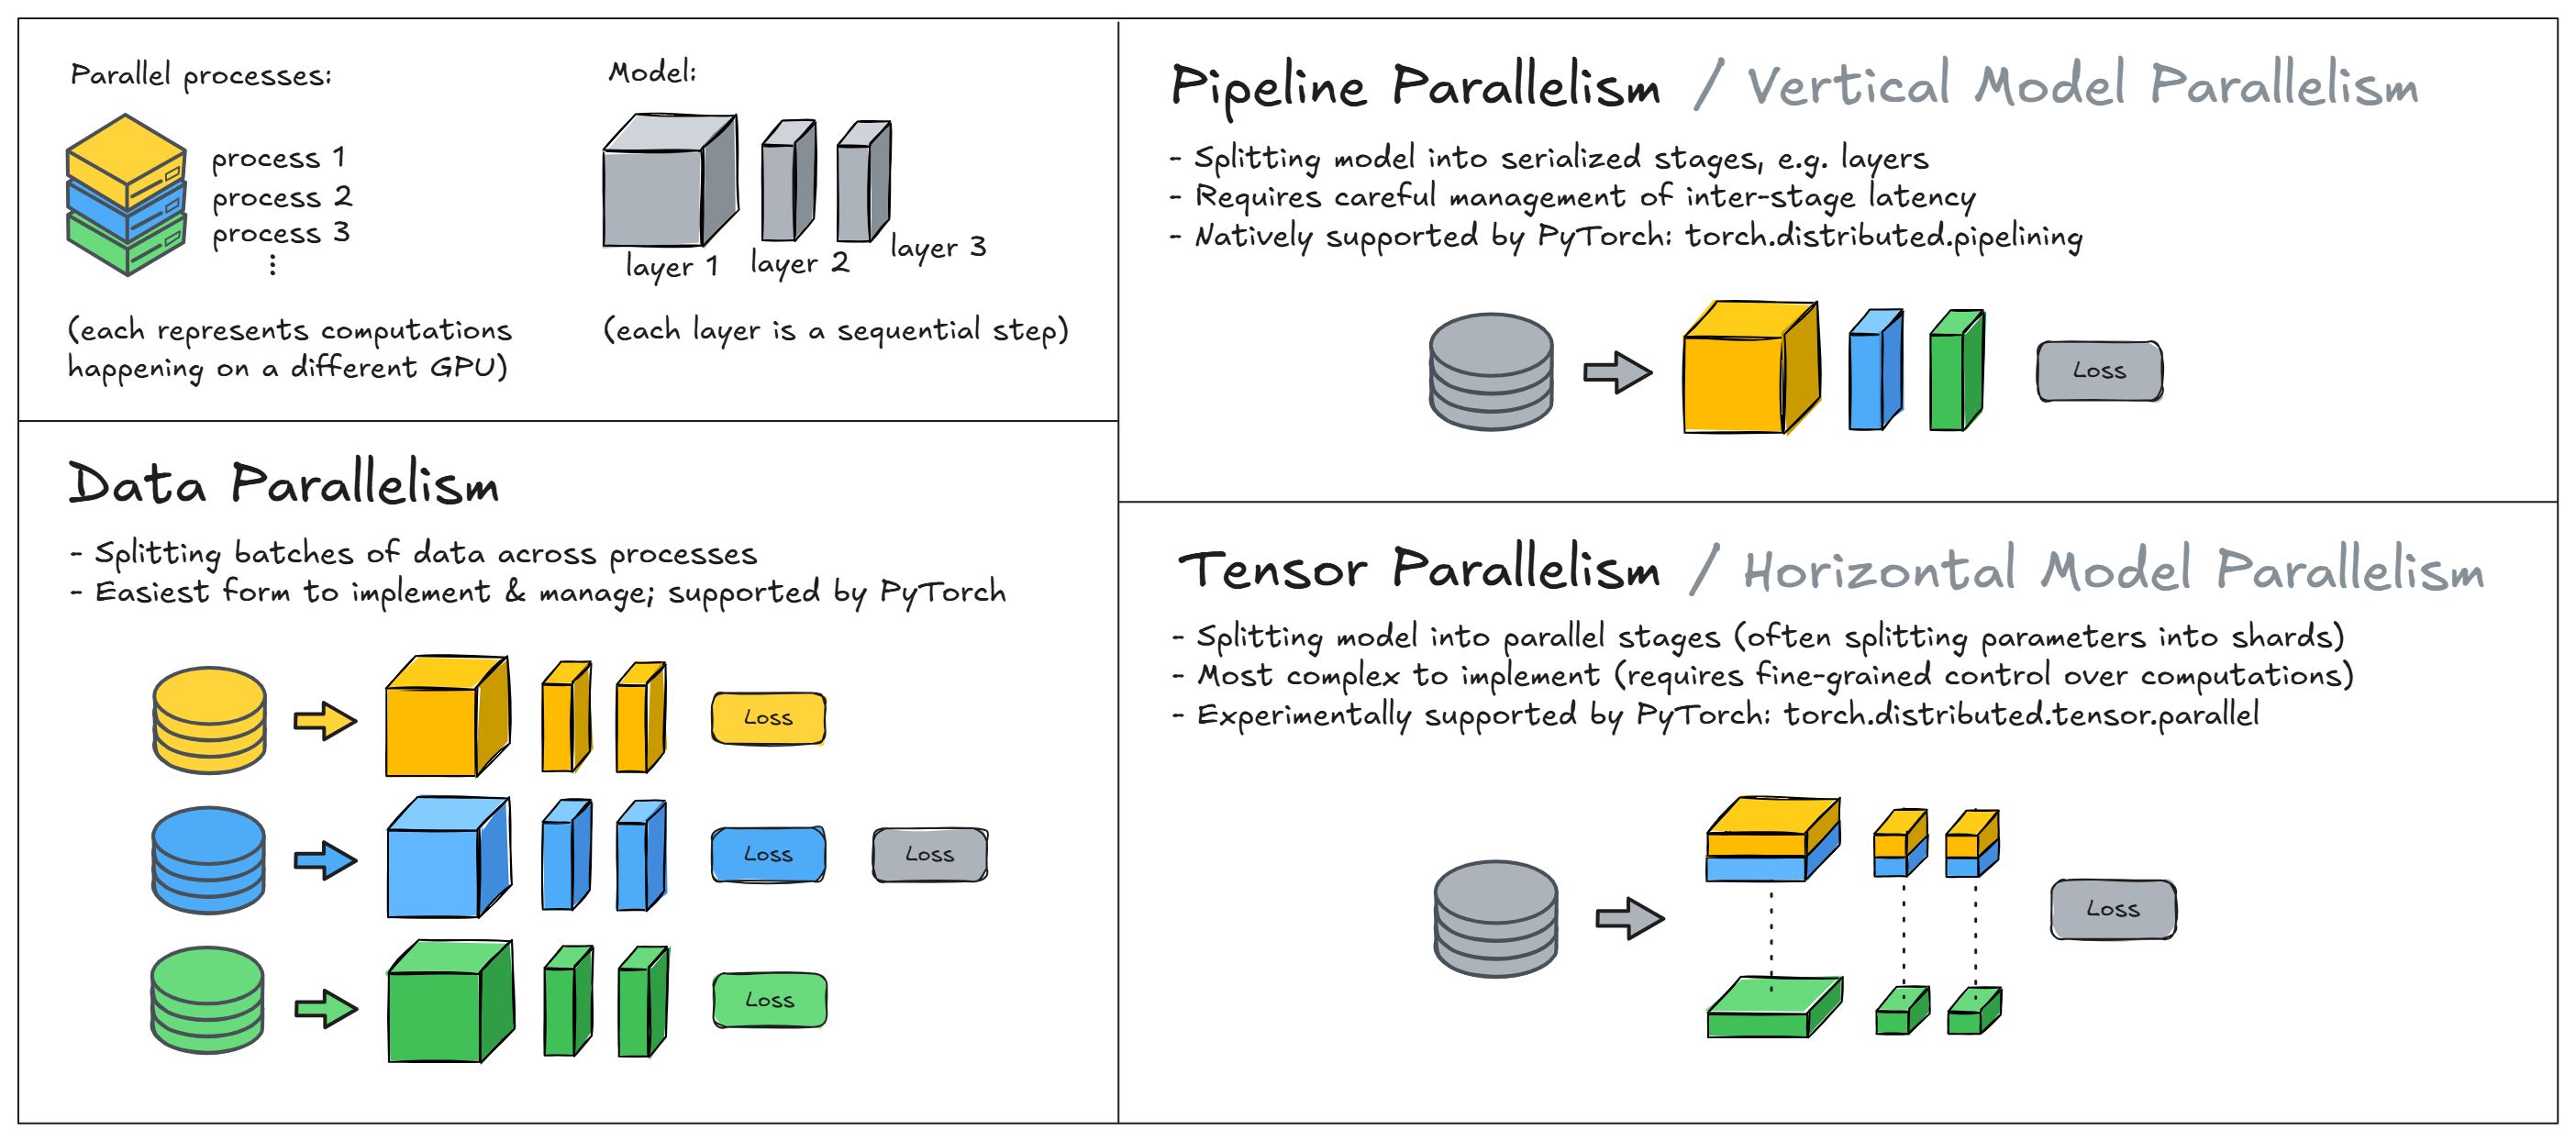
\includegraphics[width=\paperwidth]{img/parallelism.png}
    \end{frame}
% % ------------------------------------------------------------
% \begin{frame}
% \frametitle{Why distributed training?}
% \begin{itemize}
%     \item Two reasons one GPU isn't enough:
%     \begin{enumerate}
%         \item The \textbf{model} doesn't fit in GPU memory.
%         \pause
%         \item Each step is too slow --- the dataset / batch you'd like is
%         bigger than one GPU can chew.
%     \end{enumerate}
%     \pause
%     \item Three flavors of parallelism (often combined in big training runs):
% \end{itemize}
% \begin{center}
% \small
% \begin{tabular}{l l}
%     \textbf{Data parallelism}     & each worker has the full model, different data batches \\
%     \textbf{Tensor parallelism}   & split each layer's weight matrix across workers \\
%     \textbf{Pipeline parallelism} & split the layers themselves across workers (assembly line) \\
% \end{tabular}
% \end{center}
% \pause
% \vspace{0.3cm}
% \textbf{Today:} data parallelism. The other two are bigger-rig territory.
% \end{frame}

% % ------------------------------------------------------------
% \begin{frame}[fragile]
% \frametitle{Data parallelism: collectives $\to$ DDP}
% \begin{columns}
% \column{0.42\textwidth}
% \begin{tikzpicture}[scale=0.85, every node/.style={font=\scriptsize}]
%     \foreach \i/\ang in {0/90, 1/0, 2/-90, 3/180} {
%         \node[draw, circle, fill=blue!15, minimum size=0.9cm] (g\i) at (\ang:1.5) {GPU \i};
%     }
%     \draw[->, thick] (g0) to[bend left=20] (g1);
%     \draw[->, thick] (g1) to[bend left=20] (g2);
%     \draw[->, thick] (g2) to[bend left=20] (g3);
%     \draw[->, thick] (g3) to[bend left=20] (g0);
%     \node at (0,-2.3) {ring all-reduce};
% \end{tikzpicture}
% \column{0.58\textwidth}
% \begin{itemize}
%     \scriptsize
%     \item Each worker has a full model replica.
%     \pause
%     \item \textbf{Init:} broadcast weights from rank 0.
%     \pause
%     \item \textbf{Each step:} forward + backward locally on its own
%     mini-batch, then \textbf{all-reduce} gradients across all workers
%     (everyone ends up with the sum / mean), then optimizer step.
%     \pause
%     \item Ring all-reduce is bandwidth-optimal: each GPU only ever talks
%     to its two neighbors.
% \end{itemize}
% \end{columns}
% \pause
% \vspace{0.2cm}
% \begin{block}{One line of PyTorch}
% \begin{lstlisting}
% model = torch.nn.parallel.DistributedDataParallel(model)
% \end{lstlisting}
% \end{block}
% DDP wraps all the collectives behind the scenes.
% \end{frame}

% ------------------------------------------------------------
\begin{frame}
\small{
\frametitle{Glossary}
\begin{itemize}
    \item \textbf{Optimizer}: the rule for turning $\nabla \mathcal{L}$ into a parameter update.
    \item \textbf{Learning rate} $\alpha$: step size. The most important dial.
    \item \textbf{Momentum} ($\mu$): exponentially weighted average of past gradients.
    \item \textbf{Weight decay} ($\lambda$): shrink parameters toward zero each step.
    \item \textbf{Adam}: momentum + per-parameter adaptive LR + bias correction.
    \item \textbf{AdamW}: Adam with decoupled weight decay. Use by default.
    \item \textbf{LR schedule}: warmup then decay; pretty much always.
    \item \textbf{Parameter group}: subset of parameters with its own LR / weight decay.
    \item \textbf{WandB}: experiment-tracking dashboard
    \item \textbf{Sweep}: automated hyperparameter search
    % \item \textbf{Hyperband}: early termination of bad runs in a sweep.
    % \item \textbf{Data parallelism}: same model, different data per worker.
    % \item \textbf{All-reduce}: collective op --- everyone ends up with the sum.
    % \item \textbf{DDP} (\texttt{DistributedDataParallel}): PyTorch's data-parallel wrapper.

    % \hspace{0pt}
    % \rule{0.3\textwidth}{0.5pt}
    % \vspace{0.1cm}

    % \footnotesize{Today's point: knowing \emph{why} each piece exists is what
    % turns a training script that works on a toy problem into one that scales.}
\end{itemize}
}
\end{frame}

\end{document}
